\documentclass{article}

\setlength{\parindent}{0pt}

\usepackage{fullpage}
\usepackage{graphicx}

\def\Nat{{\rm I\kern-.17em N}}
\def\SFF{\hbox{I\kern-.09em\hbox{I}}}
\newcommand\Bezier{B\'{e}zier }

\newcommand\projecttitle{Ray Tracing A Messy Kitchen Counter}
\newcommand\myname{Joanne}
\newcommand\myuserid{Hong}
\newcommand\mystudentid{20470862}

\begin{document}

\begin{minipage}[t]{3in}
{\huge \bf 
	\projecttitle 
}

\medskip
Name: \myname \\ 
User ID: \myuserid \\ 
Student ID: \mystudentid 
\end{minipage}
\hfill
\begin{minipage}[t]{3in}
%%%% Use the first of these if your image is wider than tall; use the
%%%% second if your image is taller than it is wide.
\vspace{0pt}
% \includegraphics[height=2in]{image2-FRONT.png}   %%%% Change file.png to your image
\end{minipage}

\section{Mirror Reflections}
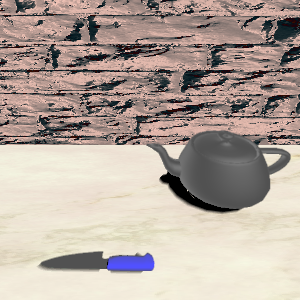
\includegraphics[width=3in]{Assets/no_reflection.png}
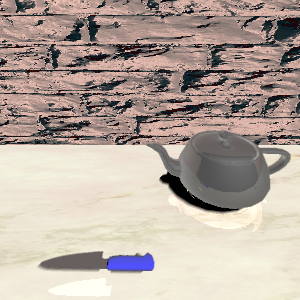
\includegraphics[width=3in]{Assets/reflection.png}

\section{Refractions}
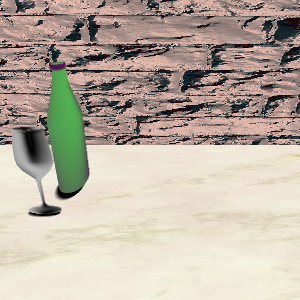
\includegraphics[width=3in]{Assets/no_refraction.png}
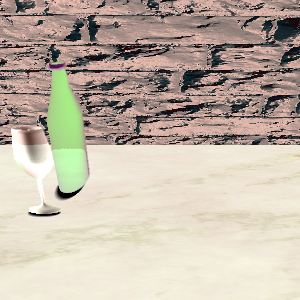
\includegraphics[width=3in]{Assets/refraction.png}

\section{Phong Shading}
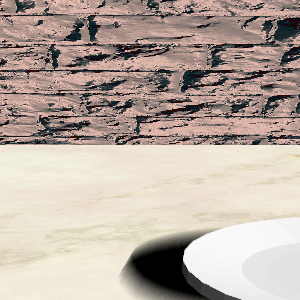
\includegraphics[width=3in]{Assets/no_phong.png}
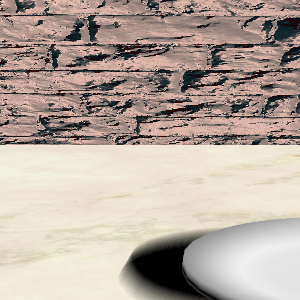
\includegraphics[width=3in]{Assets/phong.png}

\newpage

\section{Adaptive Sampling for Antialiasing}
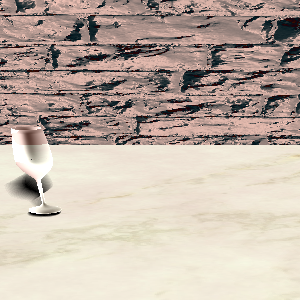
\includegraphics[width=3in]{Assets/no_antialiasing.png} \\
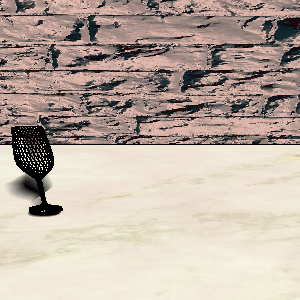
\includegraphics[width=3in]{Assets/antialiasing2.png}
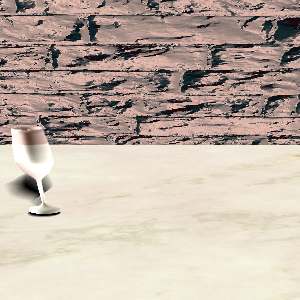
\includegraphics[width=3in]{Assets/antialiasing.png}

\section{Texture Mapping}
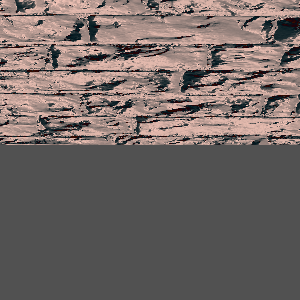
\includegraphics[width=3in]{Assets/no_texture_mapping.png}
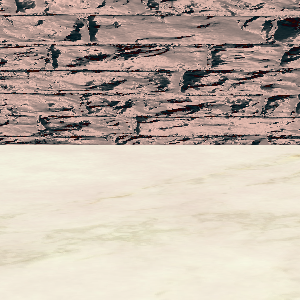
\includegraphics[width=3in]{Assets/texture_mapping.png}

\section{Bump Mapping}
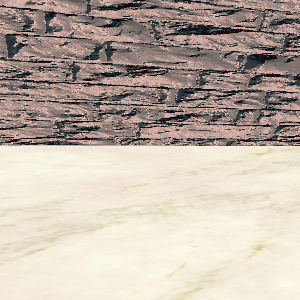
\includegraphics[width=3in]{Assets/bump_mapping.png}

\section{Soft Shadows}
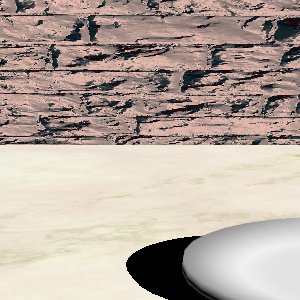
\includegraphics[width=3in]{Assets/no_soft_shadows.png}
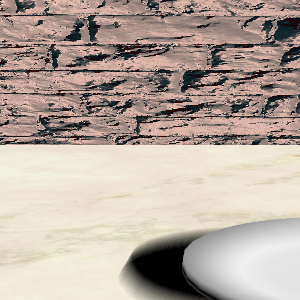
\includegraphics[width=3in]{Assets/soft_shadows.png}

\section{Constructive Solid Geometry}
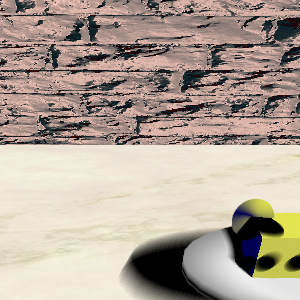
\includegraphics[width=3in]{Assets/no_csg.png}
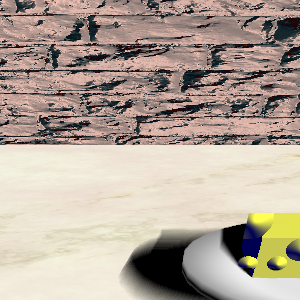
\includegraphics[width=3in]{Assets/csg.png}

\section{Gaseous Object/Particle System}
see \texttt{Assets/project.gif}

\section{Final Unique Scene}
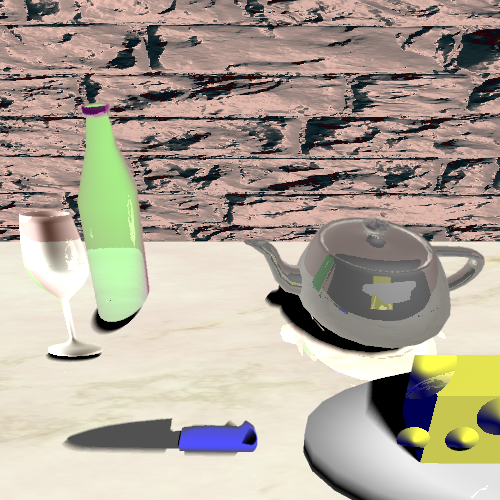
\includegraphics[width=3in]{screenshot.png}

\end{document}
